\documentclass[conference]{IEEEtran}

\usepackage{cite}
\usepackage{graphicx}

\title{Judul sementara}
\author{\IEEEauthorblockN{Muhammad Ogin Hasanuddin}\\
\IEEEauthorblockA{\textit{Fakultas Teknologi Informasi}\\
\textit{Institut Teknologi Batam}\\
Batam, Indonesia\\
moginh@iteba.ac.id}}


% START DOCUMENT
\begin{document}

% Judul
\maketitle

% Abstrak
\begin{abstract}
isi disini abstraknya dkja;sbfljkasdbfadsf
\end{abstract}

% Kata kunci
\begin{IEEEkeywords}
Firebase, Docker
\end{IEEEkeywords}

% Pendahuluan
\section{Introduction}
isi dengan introduction bahasa indonesia

contoh sitasi~\cite{brin1998anatomy, xing2004weighted}

% related works
\section{Related Works}
\subsection{PageRank Algorithm}
isi dari PageRank Algorithm


\begin{equation}
    r_j = \sum_{i \rightarrow j} \frac{r_i}{L_{out}(i)}
\end{equation}

\begin{equation}
    \sum r_i = 1
\end{equation}


\subsection{WeightedPageRank Algorithms}
isi dari WeightedPageRank Algorithms

\subsubsection{Weighted  PageRank  based  on  the  number  of  in-links  of  neighboring pages}
isi dari Weighted  PageRank  based  on  the  number  of  in-links  of  neighboring pages


\subsubsection{Weighted PageRank based on Similarity Measure}
isi dari Weighted PageRank based on Similarity Measure

\subsubsection{Weighted PageRank based on visits of links}
isi dari Weighted PageRank based on visits of links

\subsection{Hub and Authorities Algorithm}
isi dari Hub and Authorities Algorithm

\subsection{Distributed and Parallel Computing}
isi dari Distributed and Parallel Computing

% Proposed Algorithm
\section{The Proposed Algorithm}
isi dari The Proposed Algorithm

% Experiments
\section{Experiments}
isi dari Experiments

\begin{figure}
    \centering
    \def\svgwidth{\columnwidth}
    \scalebox{0.6}{\input{gambar1.pdf_tex}}
    \caption{Experiment System Architecture}
\end{figure}

\begin{figure}
    \centering
    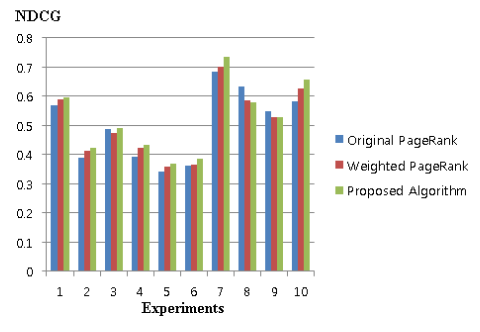
\includegraphics[width=0.4\textwidth]{gambar2.png}
    \caption{Comparison of the original PageRank and the proposed Algorithm}
\end{figure}

% Conclusions
\section{Conclusions}
isi dari Conclusions

% References
\bibliographystyle{IEEEtran}
\bibliography{IEEEabr, references}

\end{document}